%%%%%%%%%%%%%%%%%%%%%%%%%%%%%%%%%%%%%%%%%%%%%%%%%%%%%%%%%%%%%%%%%%%%%%%%%%%%%%%%
% AMS Beamer series / Bologna FC / Template
% Andrea Omicini
% Alma Mater Studiorum - Università di Bologna
% mailto:andrea.omicini@unibo.it
%%%%%%%%%%%%%%%%%%%%%%%%%%%%%%%%%%%%%%%%%%%%%%%%%%%%%%%%%%%%%%%%%%%%%%%%%%%%%%%%
%\documentclass[handout]{beamer}\mode<handout>{\usetheme{default}}
%
\documentclass[presentation, 9pt]{beamer}\mode<presentation>{\usetheme{AMSBolognaFC}}
%\documentclass[handout]{beamer}\mode<handout>{\usetheme{AMSBolognaFC}}
%%%%%%%%%%%%%%%%%%%%%%%%%%%%%%%%%%%%%%%%%%%%%%%%%%%%%%%%%%%%%%%%%%%%%%%%%%%%%%%%
\usepackage[T1]{fontenc}
\usepackage{wasysym}
\usepackage{amsmath,blkarray}
\usepackage[minted,most]{tcolorbox}
\usepackage{centernot}
\usepackage{fontawesome}
\usepackage{fancyvrb}
\setminted[scala]{fontsize=\scriptsize,baselinestretch=1,obeytabs=true, tabsize=2}
\usepackage[ddmmyyyy]{datetime}
\renewcommand{\dateseparator}{}
%\renewcommand{\thefootnote}{\fnsymbol{footnote}}
\newcommand{\version}{1}
\usepackage[
	backend=biber,
	citestyle=authoryear-icomp,
	maxcitenames=1,
	bibstyle=numeric]{biblatex}

	\makeatletter

\addbibresource{biblio.bib}
%%%%%%%%%%%%%%%%%%%%%%%%%%%%%%%%%%%%%%%%%%%%%%%%%%%%%%%%%%%%%%%%%%%%%%%%%%%%%%%%
\title[MacroSwarm]
{MacroSwarm \\ Field-based Compositional Framework for Swarm Programming}
%
%subtitle[How to build applications that span in different platforms]
%{How to build applications that span in different platforms}
%
\author[\sspeaker{Aguzzi}]
{\speaker{Gianluca Aguzzi} \href{mailto:gianluca.aguzzi@unibo.it}{gianluca.aguzzi@unibo.it}\\
\otherauthor{Roberto Casadei} \href{mailto:roby.casadei@unibo.it}{roby.casadei@unibo.it}\\
\otherauthor{Mirko Viroli} \href{mailto:mirko.viroli@unibo.it}{mirko.viroli@unibo.it}}
%
\institute[DISI, Univ.\ Bologna]
{Dipartimento di Informatica -- Scienza e Ingegneria (DISI)\\
\textsc{Alma Mater Studiorum} -- Universit{\`a} di Bologna \\[0.5cm]
\textbf{Talk @} \bold{COORDINATION 2023}

\vspace{0.2cm}
\fbox{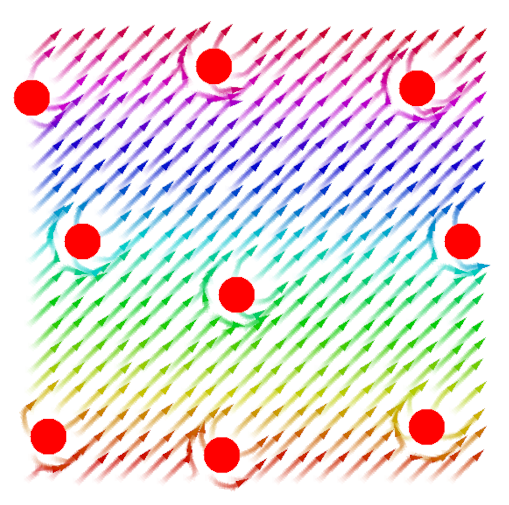
\includegraphics[width=0.2\textwidth]{img/obstacle-avoidance}}
\fbox{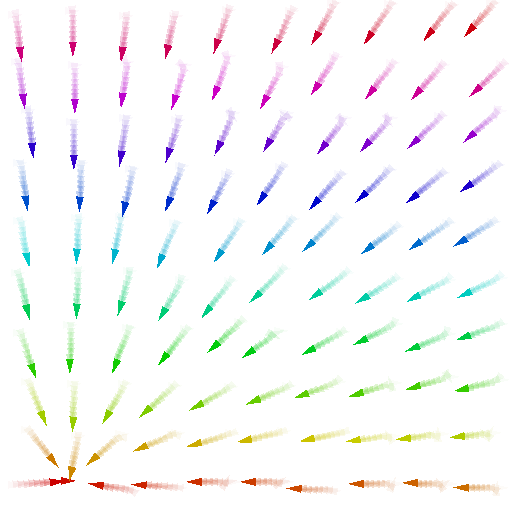
\includegraphics[width=0.2\textwidth]{img/towards-leader.png}}
\fbox{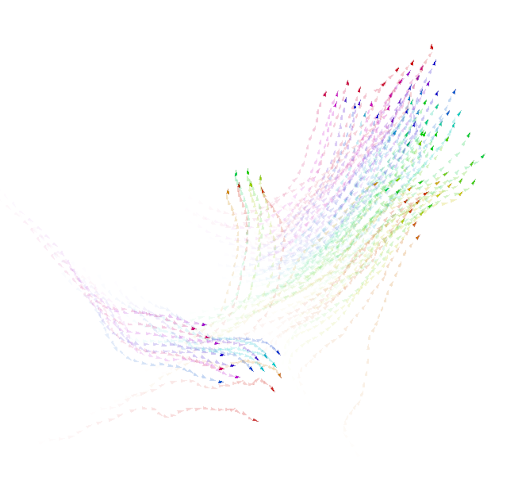
\includegraphics[width=0.2\textwidth]{img/flock.png}}
\fbox{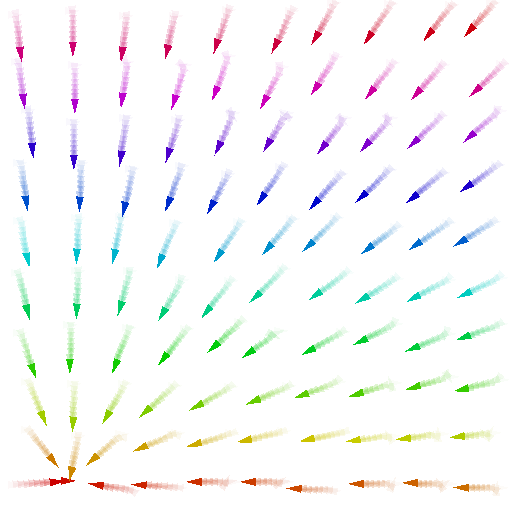
\includegraphics[width=0.2\textwidth]{img/towards-leader.png}}}
%
\renewcommand{\dateseparator}{/}
\date[\today]{}
%
\AtBeginSection[]
{
  \begin{frame}
  \frametitle{Contents}
  \tableofcontents[currentsubsection, 
	sectionstyle=show/shaded, 
	subsectionstyle=show/shaded]
  \end{frame}
}
\AtBeginSubsection[]
{
  \begin{frame}
  \frametitle{Contents}
  \tableofcontents[currentsubsection, 
	sectionstyle=show/shaded, 
	subsectionstyle=show/shaded]
  \end{frame}
}
%%%%%%%%%%%%%%%%%%%%%%%%%%%%%%%%%%%%%%%%%%%%%%%%%%%%%%%%%%%%%%%%%%%%%%%%%%%%%%%%
\begin{document}
%%%%%%%%%%%%%%%%%%%%%%%%%%%%%%%%%%%%%%%%%%%%%%%%%%%%%%%%%%%%%%%%%%%%%%%%%%%%%%%%

%/////////
\frame{\titlepage}
%/////////

%===============================================================================
\begin{frame}{Context}
\centering
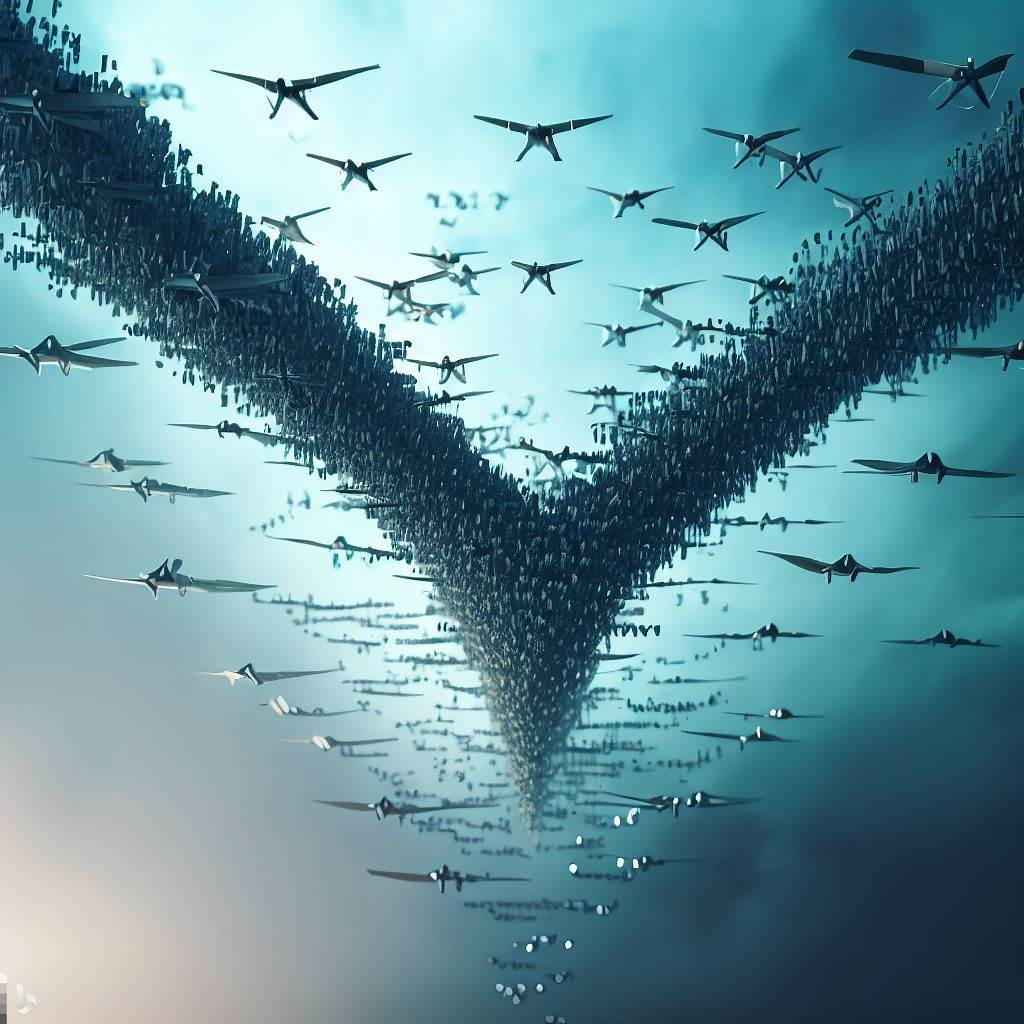
\includegraphics[width=0.55\textwidth]{img/flock.jpeg}
\\
\huge{\emph{Networked Mobile Nodes}} \faPlus \, \textbf{Collective Behaviours}
\end{frame}
\begin{frame}{Swarm Behaviours}
A \emph{swarm behaviour} is a \emph{collective} behaviour that emerges from the \emph{local} interactions of a \emph{population} of \emph{autonomous} entities.
\begin{alertblock}{In a nutshell}
\begin{itemize}
	\item \emph{Emergent} \faArrowRight \, \emph{self-organisation} and \emph{self-adaptation}
	\item \emph{Decentralised} \faArrowRight \, \emph{locality} and \emph{scalability}
	\item \emph{Asynchronous} \faArrowRight \, \emph{robustness} and \emph{fault-tolerance}
\end{itemize}	
\end{alertblock}
\end{frame}
\begin{frame}{Programming Swarm Behaviours}

\end{frame}
\begin{frame}{MacroSwarm}

\end{frame}
\begin{frame}{Aggregate Computing}
\begin{alertblock}{In a nutshell}
\begin{itemize}
	\item \emph{Computational fields} as first-class abstractions
	\item Programs as field transformations through \emph{field calculus} 
	\item Inspiration from co-fields and artificial pontential fields
\end{itemize}
\end{alertblock}
\begin{block}{Why}
\begin{itemize}
	\item \emph{Top-down behaviour-based design} \faArrowRight \, \emph{compositionality} and \emph{collective stance} of aggregate computing;
	\item \emph{Scalability} \faArrowRight fully decentralised and asynchronous
	\item \emph{Formal approach} \faArrowRight \, based on the field calculus
		
	\item \emph{Pragmatism} \faArrowRight \, witnessed by open-source, maintained, concrete software artefacts like the ScaFi DSL, Alchemist and {\sc{}ScaFi-Web}
	\item \emph{Operational flexibility} \faArrowRight \, supporting different architectural styles and execution policies.
\end{itemize}
\end{block}
\end{frame}

\begin{frame}{Architecture}
\centering
\fbox{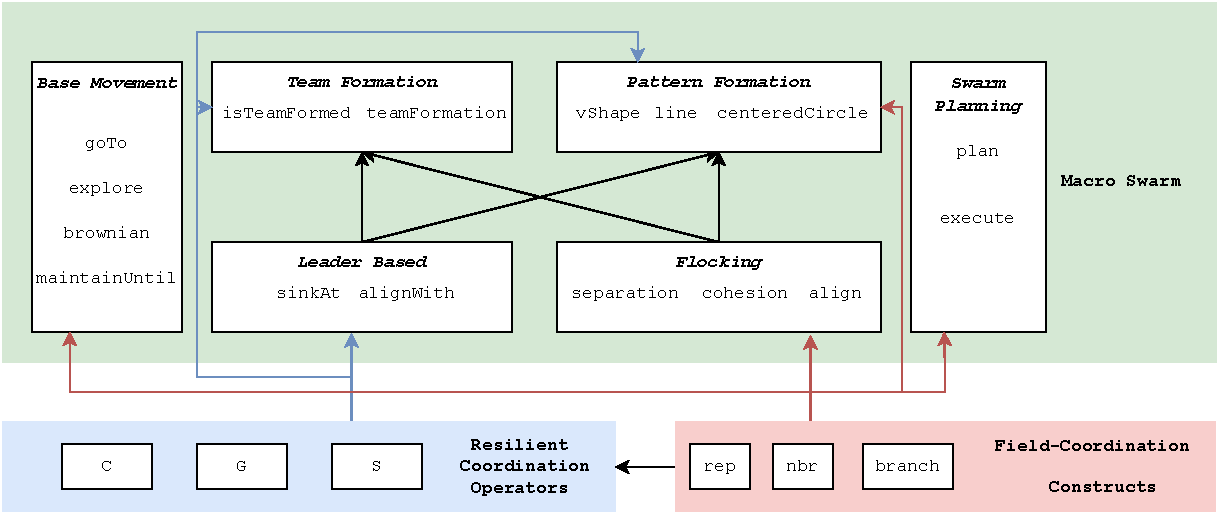
\includegraphics[width=0.98\textwidth]{img/architecture.drawio.pdf}}
\end{frame}

%===============================================================================
\section*{}
%===============================================================================

%/////////
\frame{\titlepage}
%/////////

%===============================================================================
\section*{\refname}
%===============================================================================

%%%%
\setbeamertemplate{page number in head/foot}{}
%/////////
\begin{frame}[c,noframenumbering, allowframebreaks]{\refname}
%\begin{frame}[t,allowframebreaks,noframenumbering]{\refname}
	\tiny
	\printbibliography
\end{frame}
%/////////

%%%%%%%%%%%%%%%%%%%%%%%%%%%%%%%%%%%%%%%%%%%%%%%%%%%%%%%%%%%%%%%%%%%%%%%%%%%%%%%%
\end{document}
%%%%%%%%%%%%%%%%%%%%%%%%%%%%%%%%%%%%%%%%%%%%%%%%%%%%%%%%%%%%%%%%%%%%%%%%%%%%%%%%
